%!TeX program = xelatex
% 闫达的个人简历 (Curriculum Vitae)
% Email: alexyan1987@outlook.com / yanda@wmu.edu.cn
% Web: https://870603.xyz
% Repo: https://github.com/fabea87/cv

\documentclass[12pt,a4paper]{report}

\usepackage{fontspec}
\usepackage{xeCJK}
\usepackage[english]{babel}
\usepackage{csquotes}
\usepackage{microtype}
\usepackage{datetime}
\usepackage{hyperref}
\usepackage{geometry}
\usepackage{enumitem}
\usepackage{needspace}
\usepackage{setspace}
\usepackage[dvipsnames,table]{xcolor}
\usepackage{graphicx}
\usepackage{fontawesome5}
\usepackage{academicons}
\usepackage{fancyhdr}
\usepackage{lastpage}
\usepackage{booktabs}
\usepackage{array}

% Accent color: Vibrant Royal Blue (#1A56B2)
\definecolor{cvaccent}{HTML}{1A56B2}

% select default typefaces
\setmainfont{RobotoCondensed}[
  Path = fonts/,
  Extension = .ttf,
  Ligatures = TeX,
  UprightFont = *-Regular,
  BoldFont = *-Medium,
  ItalicFont = *-Italic,
  BoldItalicFont = *-MediumItalic
]

% Body CJK face. Use the STATIC Noto Serif CJK SC family (font-noto-serif-cjk-sc),
% which ships real Regular / Bold / Light faces.
% Do NOT use the variable "Noto Serif SC" (NotoSerifSC[wght].ttf): it has no separate
% bold face, and XeTeX ignores the wght axis, so any name- or pattern-based bold
% request silently renders the Regular weight.
\setCJKmainfont{Noto Serif CJK SC}[
  BoldFont           = {Noto Serif CJK SC Bold},
  ItalicFont         = {Noto Serif CJK SC},
  ItalicFeatures     = {FakeSlant = 0.2},
  BoldItalicFont     = {Noto Serif CJK SC Bold},
  BoldItalicFeatures = {FakeSlant = 0.2}
]

\newfontfamily\headingfont{RobotoCondensed}[
  Path = fonts/,
  Extension = .ttf,
  Ligatures = TeX,
  Scale = 1.05,
  UprightFont = *-Regular,
  BoldFont = *-Bold,
  SemiBoldFont = *-SemiBold,
  MediumFont = *-Medium
]

% CJK heading face: 汇文正楷 (Huiwen ZhengKai), the ONLY CJK heading face.
% Single Regular weight, so fake bold supplies the \bfseries used by \namefont
% and the section headings. The TTF is NOT in git (personal-use licence, no
% redistribution), so it must be supplied at build time: locally by dropping
% fonts/HuiwenZhengKai.ttf into place, in CI by the HUIWEN_FONT_B64 secret.
% There is deliberately NO fallback font -- a missing file is a hard error.
\IfFileExists{fonts/HuiwenZhengKai.ttf}{}{%
  \errmessage{*** CV-cn.tex requires fonts/HuiwenZhengKai.ttf (\string\cjkheadingfont)
    -- 汇文正楷 is not distributed with this repo. Place the TTF in fonts/ (local)
    or set the HUIWEN_FONT_B64 repository secret (CI). ***}%
}
\newCJKfontfamily\cjkheadingfont{HuiwenZhengKai}[
  Path = fonts/,
  Extension = .ttf,
  AutoFakeBold = 2.0
]

% what is your name?
\newcommand{\myname}{闫\hspace{0.5em}达\texorpdfstring{\Large{ 博士}}{ 博士}}

% how far to tab for list items with left-aligned date
\newcommand{\listtabwidth}{1.7cm}

% define font to use as document's title
\newcommand{\namefont}[1]{{\cjkheadingfont\bfseries\Huge\color{cvaccent}{#1}}}

% set page margins
\geometry{left=0.62in, right=0.58in, top=0.50in, bottom=0.50in}

% prevent paragraph indentation
\setlength\parindent{0em}

% set line spacing
\setstretch{0.82}

% define space between list items
\newcommand{\listitemspace}{0.12em}

% right-aligned publication tag
\newcommand{\pubtag}[1]{\hspace*{\fill}\mbox{(#1)}}

% Thoughteer-inspired section heading: colored flanking lines + heading
\newcounter{cvsection}
\newcommand{\cvsection}[1]{%
  \Needspace{6\baselineskip}%
  \par\vspace{10pt plus 2pt minus 2pt}%
  \refstepcounter{cvsection}%
  \noindent
  \textcolor{cvaccent}{%
    \rule[0.55ex]{\listtabwidth}{0.85pt}%
    \hspace{0.6em}%
    {\headingfont\cjkheadingfont\bfseries\large\ifnum\value{cvsection}<10 0\fi\arabic{cvsection}\hspace{0.5em}#1}%
    \hspace{0.6em}%
    \leaders\hrule height \dimexpr 0.55ex + 0.85pt\relax depth -0.55ex\hfill\kern0pt
  }\par
  \vspace{0.25em}%
  \nopagebreak
}

% make unordered lists without bullets and use compact spacing
\renewenvironment{itemize}
{
  \begin{list}{}{\setlength{\leftmargin}{0em}
      \setlength{\parskip}{0em}
      \setlength{\itemsep}{\listitemspace}
  \setlength{\parsep}{\listitemspace}}}
  {
\end{list}}

% make lists with consistent hanging indent
\newlist{tablist}{description}{3}
\setlist[tablist]{%
  leftmargin=\listtabwidth,
  labelwidth=\dimexpr\listtabwidth - 0.15cm\relax,
  labelsep=0.15cm,
  itemindent=0pt,
  topsep=0em,
  partopsep=0em,
  itemsep=\listitemspace,
  parsep=\listitemspace,
  align=left,
  font=\normalfont
}

% make compact enumerated lists
\setlist[enumerate]{topsep=0.10em, partopsep=0em, itemsep=\listitemspace, parsep=\listitemspace, leftmargin=1.6em, font=\normalfont}

% date format
\newcommand{\edittoday}{\number\year 年\number\month 月}

% define hyperlink appearance and metadata for pdf properties
\hypersetup{
  colorlinks   = true,
  urlcolor     = cvaccent,
  citecolor    = black,
  linkcolor    = cvaccent,
  pdfauthor    = {闫达},
  pdfkeywords  = {应用语言学, 翻译学, 形成性评估, 计算机辅助教学, 人工智能},
  pdftitle     = {闫达：个人简历},
  pdfsubject   = {个人简历},
  pdfpagemode  = UseNone
}

% page footer with update date, name and page numbers
\pagestyle{fancy}
\fancyhf{}
\renewcommand{\headrulewidth}{0pt}
\fancyfoot[L]{\footnotesize\color{black!70}更新时间：\edittoday}
\fancyfoot[R]{\footnotesize\color{black!70}闫达 --- 第 \thepage{} / \pageref{LastPage} 页}

\begin{document}
\raggedright{}

% display your name, institution, contact info and photo
\begin{minipage}[t]{0.73\textwidth}
  \vspace{0pt}%
  \namefont{\myname}\\[0.40em]
  {\normalsize\faUniversity\hspace{0.35em}温州医科大学}\\[0.22em]
  {\normalsize\faBuilding[regular]\hspace{0.4em}外国语学院}\\[0.50em]
  \href{mailto:alexyan1987@outlook.com}{\faEnvelope[regular]\hspace{0.4em}alexyan1987@outlook.com}\hspace{1.4em}%
  \href{mailto:yanda@wmu.edu.cn}{\faEnvelope[regular]\hspace{0.4em}yanda@wmu.edu.cn}\\[0.30em]
  \href{tel:+8618569800613}{\faWhatsapp\hspace{0.4em}+86 185 6980 0613}\hspace{1.4em}%
  \href{https://870603.xyz}{\faGlobe\hspace{0.35em}870603.xyz}\hspace{1.4em}%
  {\normalsize%
    \href{https://orcid.org/0000-0002-1265-9772}{\aiOrcid}\hspace{0.35em}%
    \href{https://scholar.google.com/citations?user=28WTkNkAAAAJ&hl=en}{\aiGoogleScholar}\hspace{0.35em}%
    \href{https://www.webofscience.com/wos/author/record/AAE-3520-2022}{\aiClarivate}\hspace{0.35em}%
    \href{https://www.scopus.com/authid/detail.uri?authorId=57192956833}{\aiScopus}%
  }
\end{minipage}\hfill
\begin{minipage}[t]{0.24\textwidth}
  \vspace{0pt}%
  \raggedleft
  % keep a 1cm gap on the right so the portrait sits further left
  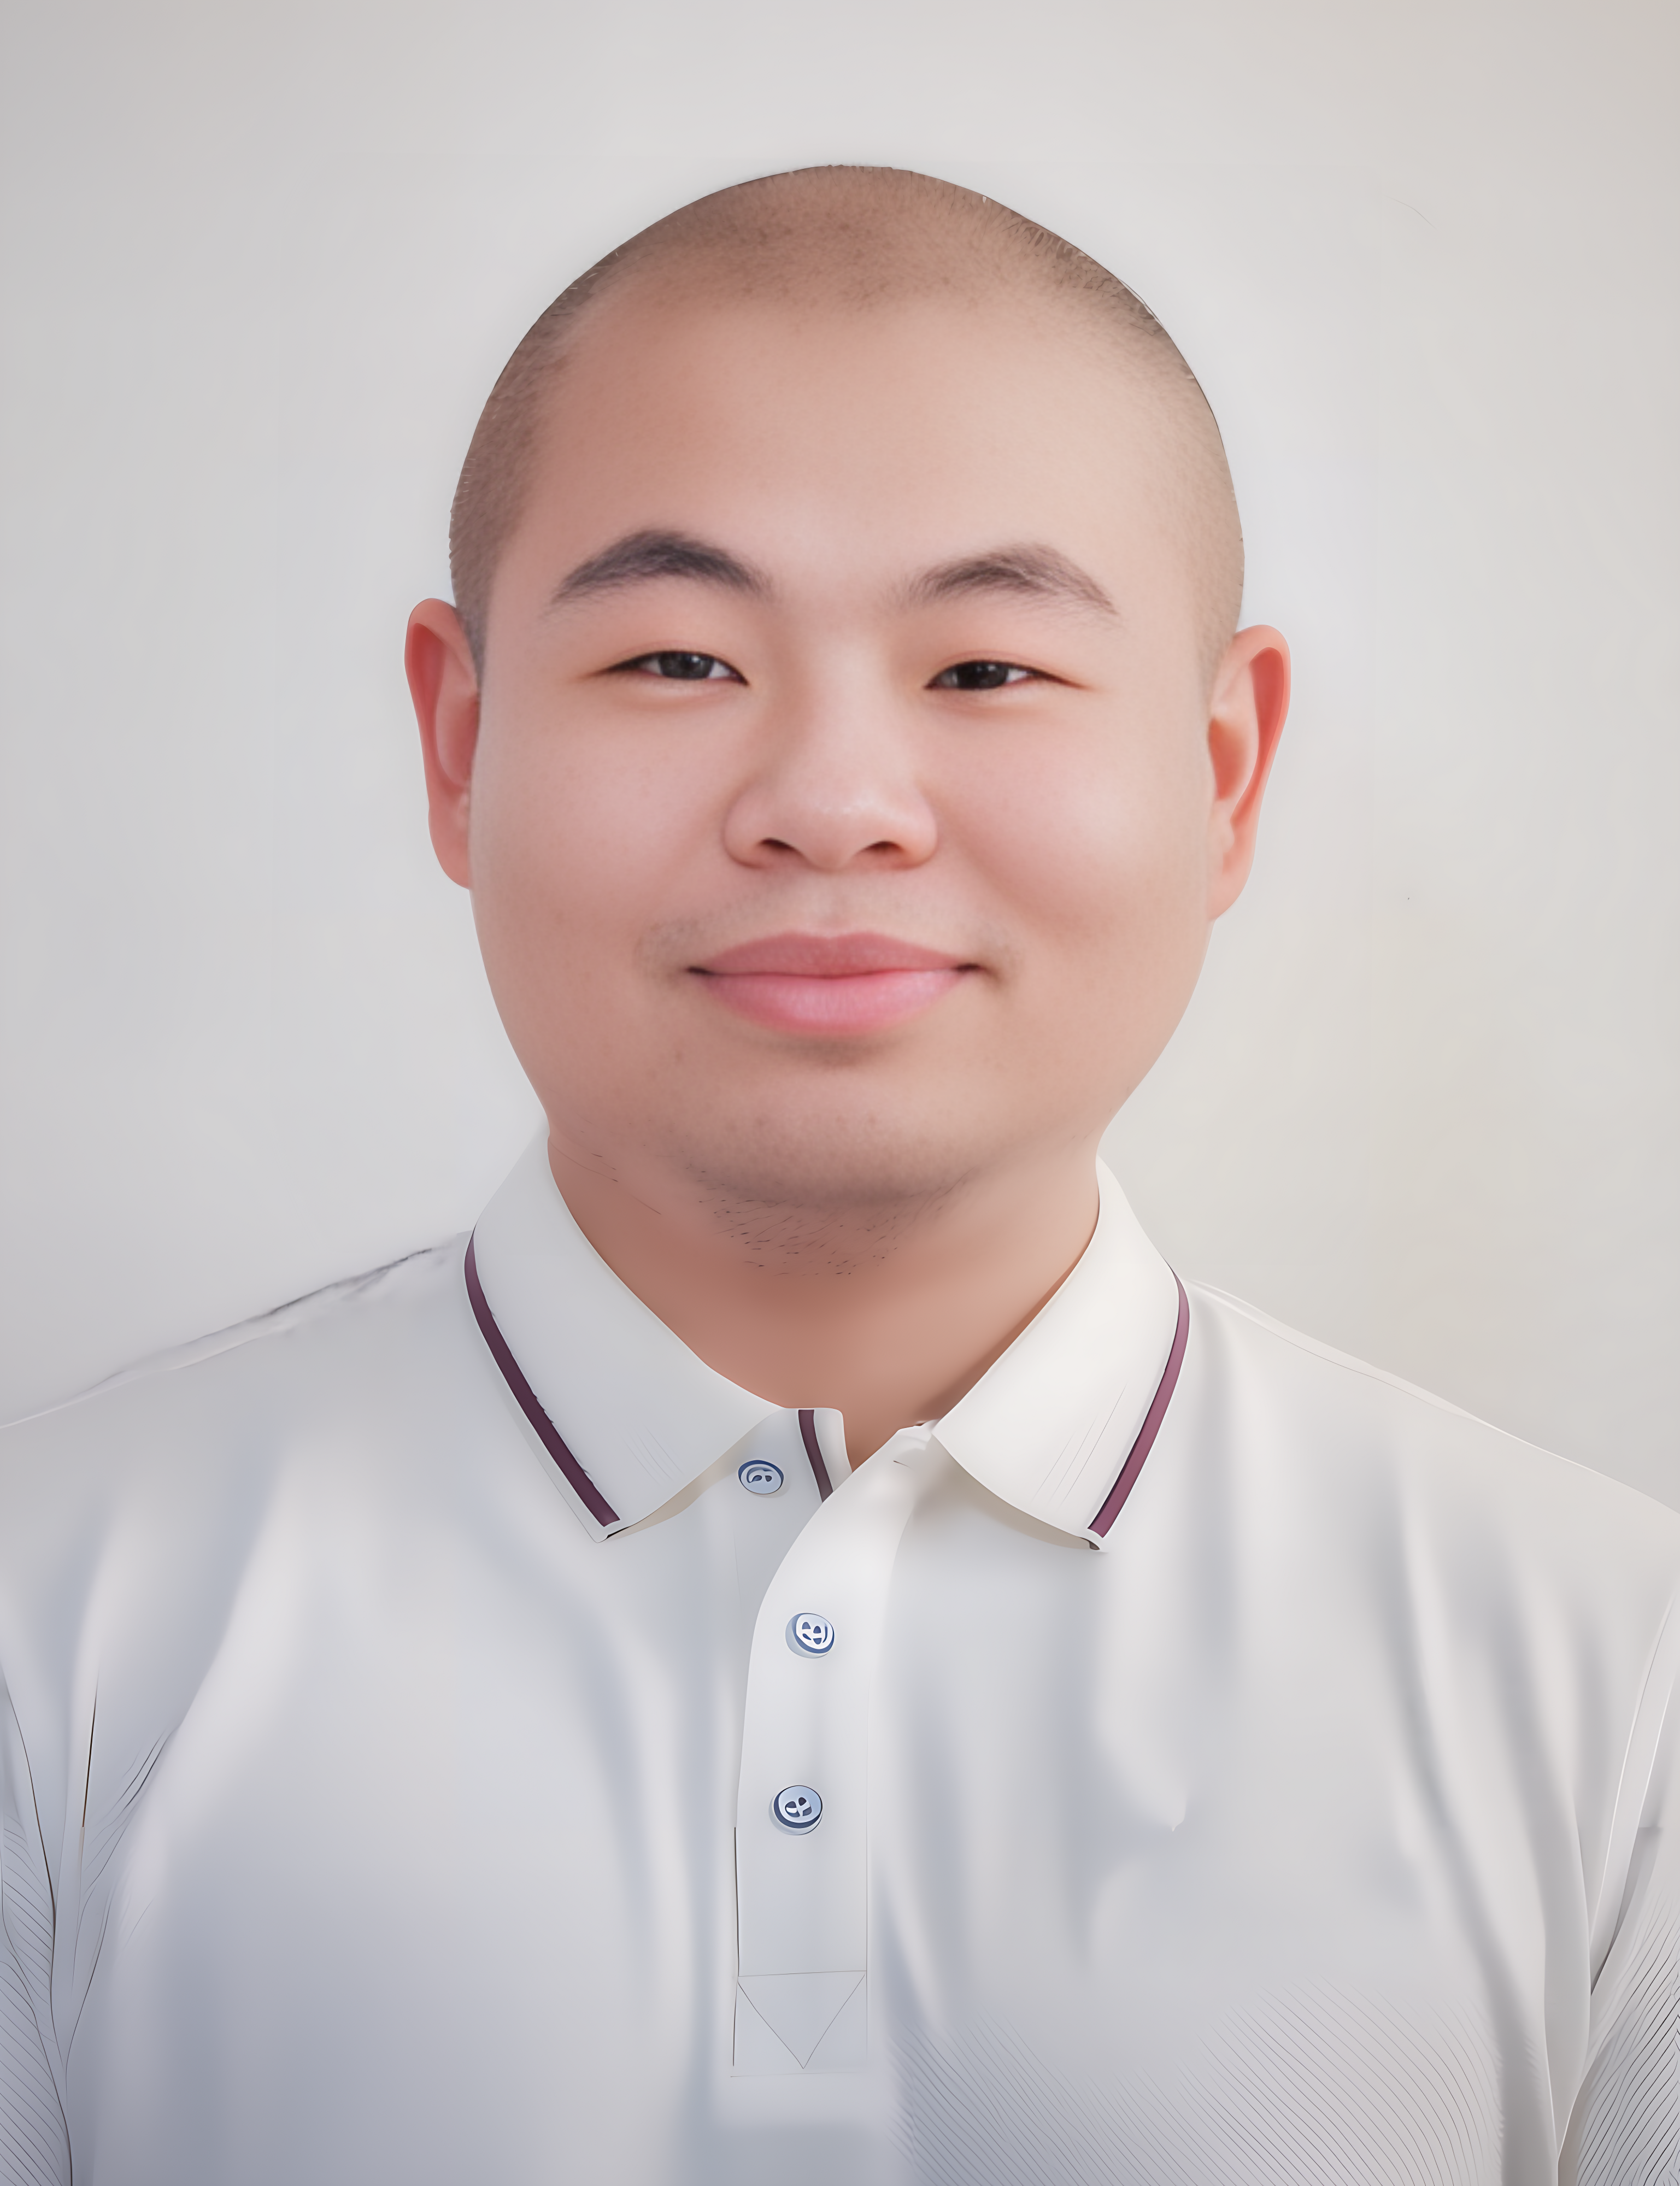
\includegraphics[width=2.55cm, height=3.35cm, keepaspectratio]{photo_up.png}\hspace*{1cm}%
\end{minipage}

\cvsection{教育背景}

\begin{tablist}
\item[博士] \textbf{翻译学}，马来西亚理科大学 语言、文学与翻译学院，2025
\item[硕士] \textbf{翻译学}，温州大学 外国语学院，2013
\item[学士] \textbf{英语专业}，河南科技大学 外国语学院，2008
\end{tablist}

\cvsection{任职经历}

\begin{tablist}
\item[2026--] \textbf{副研究员}，温州医科大学
\item[2025--26] \textbf{讲师}，温州医科大学 外国语学院
\item[2020--25] \textbf{讲师}，信阳农林学院 外国语学院
\item[2013--20] \textbf{助教}，信阳农林学院 外国语学院
\end{tablist}

\cvsection{研究方向}

\begin{enumerate}[itemsep=0.04em, parsep=0.04em, topsep=0.08em]
  \item \textbf{应用语言学}与外语教学法。
  \item \textbf{计算机辅助语言学习}与口笔译技术培训。
  \item 二语习得中的教学与\textbf{形成性反馈}。
  \item \textbf{人机交互}在教育反馈、高等教育与语言教学中的应用。
\end{enumerate}

\cvsection{发表论文}

\begin{tablist}
\item[2026] \textbf{Yan, D.*} Metacognitive instruction to enhance EFL writers' metacognition, feedback uptake, and revision performance in a GenAI-assisted feedback context. \textit{International Journal of Applied Linguistics}. Advance online publication.~\href{https://doi.org/10.1111/ijal.70328}{\aiDoi} \pubtag{SSCI一区}

\item[2026] \textbf{Yan, D.*}, Kasuma, S. A. A., \& Amini, M. Revisiting dialogic feedback in the age of GenAI: An investigation into L2 writers' feedback seeking interactions. In \textit{Generative AI in Education: Theories, Applications, and Ethical Frontiers} (pp. 261--281). Springer.~\href{https://doi.org/10.1007/978-981-95-4871-2_14}{\aiDoi} \pubtag{图书章节}

\item[2026] Tian, F., \textbf{Yan, D.}, \& Umar, I. N. Bridging language and discipline: The impact of digital game-based learning on technical vocabulary acquisition and motivation. \textit{Journal of Educational Computing Research}, \textit{64}(4), 791--820.~\href{https://doi.org/10.1177/07356331251414550}{\aiDoi} \pubtag{SSCI一区}

\item[2025] \textbf{Yan, D.*}, Tian, F., Li, H., Yu, G., \& Li, J. A GenAI-supported dialogic model to enhance the functions of peer feedback in EFL writing: A mixed-method interventional study. \textit{System}, \textit{136}, Article 103895.~\href{https://doi.org/10.1016/j.system.2025.103895}{\aiDoi} \pubtag{SSCI一区}

\item[2025] \textbf{Yan, D.*}, \& Yu, G. Effects of interactive vs. complementary approaches to integrating automated and peer feedback on L2 writers' feedback quality and performance improvement. \textit{Computer Assisted Language Learning}. Advance online publication, 1--24.~\href{https://doi.org/10.1080/09588221.2025.2569352}{\aiDoi} \pubtag{SSCI一区}

\item[2025] \textbf{Yan, D.*}, Jia, C., \& Tian, F. Automated feedback complements online dialogic peer feedback: Fostering L2 writers' feedback quality and self-regulatory writing strategy use. \textit{Interactive Learning Environments}, \textit{33}(10), 6021--6035.~\href{https://doi.org/10.1080/10494820.2025.2491620}{\aiDoi} \pubtag{SSCI一区}

\item[2025] \textbf{Yan, D.}, \& Jia, C.* Occupational stress and turnover intentions among simultaneous interpreters: The mediating role of burnout and the moderating role of grit. \textit{Perspectives: Studies in Translation Theory and Practice}, \textit{34}(5), 1025--1040.~\href{https://doi.org/10.1080/0907676X.2025.2478403}{\aiDoi} \pubtag{A\&HCI, SSCI二区}

\item[2024] \textbf{Yan, D.} Comparing individual vs. collaborative processing of ChatGPT-generated feedback: Effects on L2 writing task improvement and learning. \textit{Language Learning \& Technology}, \textit{28}(1), 1--19.~\href{https://doi.org/10.64152/10125/73597}{\aiOpenAccess\hspace{0.25em}\aiDoi} \pubtag{SSCI一区}

\item[2024] \textbf{Yan, D.}, \& Zhang, S.* L2 writer engagement with automated written corrective feedback provided by ChatGPT: A mixed method multiple case study. \textit{Humanities and Social Sciences Communications}, \textit{11}(1), Article 1086.~\href{https://doi.org/10.1057/s41599-024-03543-y}{\aiOpenAccess\hspace{0.25em}\aiDoi} \pubtag{SSCI一区, A\&HCI}

\item[2024] \textbf{Yan, D.} Rubric co-creation to promote quality, interactivity, and uptake of peer feedback. \textit{Assessment \& Evaluation in Higher Education}, \textit{49}(8), 1017--1034.~\href{https://doi.org/10.1080/02602938.2024.2333005}{\aiDoi} \pubtag{SSCI一区}

\item[2024] \textbf{Yan, D.} Feedback seeking abilities of L2 writers using ChatGPT: A mixed method multiple case study. \textit{Kybernetes}, \textit{54}(7), 3757--3781.~\href{https://doi.org/10.1108/K-09-2023-1933}{\aiDoi} \pubtag{SCI二区}

\item[2023] \textbf{Yan, D.}, Kasuma, S. A. A., \& Amini, M. Gender difference in digital literacy among translation trainees: Self-perceptions and application abilities. \textit{International Journal of Academic Research in Progressive Education and Development}, \textit{12}(3), 2393--2899.~\href{https://doi.org/10.6007/IJARPED/v12-i3/19611}{\aiOpenAccess\hspace{0.25em}\aiDoi} \pubtag{ERA}

\item[2023] \textbf{Yan, D.}, Kasuma, S. A. A., \& Amini, M. Status quo of the formative assessment enactments in spoken language interpreter training: A scoping review of research and practice. \textit{International Journal of Academic Research in Progressive Education and Development}, \textit{12}(4), 652--673.~\href{https://doi.org/10.6007/IJARPED/v12-i4/19884}{\aiOpenAccess\hspace{0.25em}\aiDoi} \pubtag{ERA}

\item[2023] Gong, H., \& \textbf{Yan, D.*} The impact of Danmaku-based and synchronous peer feedback on L2 oral performance: A mixed-method investigation. \textit{PLOS ONE}, \textit{18}(4), Article e0284843.~\href{https://doi.org/10.1371/journal.pone.0284843}{\aiOpenAccess\hspace{0.25em}\aiDoi} \pubtag{SCI一区}

\item[2023] \textbf{Yan, D.} Impact of ChatGPT on learners in a L2 writing practicum: An exploratory investigation. \textit{Education and Information Technologies}, \textit{28}(11), 13943--13967.~\href{https://doi.org/10.1007/s10639-023-11742-4}{\aiDoi} \pubtag{SSCI一区}

\item[2022] \textbf{Yan, D.}, \& Fan, Q. Online informal learning community for interpreter training amid COVID-19: A pilot evaluation. \textit{PLOS ONE}, \textit{17}(11), Article e0277228.~\href{https://doi.org/10.1371/journal.pone.0277228}{\aiOpenAccess\hspace{0.25em}\aiDoi} \pubtag{SCI一区}

\item[2022] \textbf{Yan, D.}, \& Wang, J. Teaching data science to undergraduate translation trainees: Pilot evaluation of a task-based course. \textit{Frontiers in Psychology}, \textit{13}, Article 939689.~\href{https://doi.org/10.3389/fpsyg.2022.939689}{\aiOpenAccess\hspace{0.25em}\aiDoi} \pubtag{SSCI二区}

\item[2022] \textbf{Yan, D.} Review of the book \textit{Cognitive bases of second language fluency}, Norman Segalowitz (Ed.). \textit{Porta Linguarum}, \textit{38}.~\href{https://doi.org/10.30827/portalin.vi38.23934}{\aiOpenAccess\hspace{0.25em}\aiDoi} \pubtag{SSCI二区, 书评}

\item[2018] 杨明星, 吴丽华, 牛桂玲, \& \textbf{闫达}. “互联网+”背景下多模态, 多语种外交话语平行语料库设计与创建探析. \textit{外语教学}, \textit{39}(6), 13--19. \pubtag{CSSCI}

\item[2016] Yang, M., \& \textbf{Yan, D.} The translation strategies for Chinese diplomatic neologisms from the perspective of ``Political Equivalence''. \textit{Babel}, \textit{62}(4), 661--675.~\href{https://doi.org/10.1075/babel.62.4.07yan}{\aiDoi} \pubtag{SSCI三区, A\&HCI}

\item[2013] 杨明星, \& \textbf{闫达}. 现代信息技术条件下外交机辅翻译模型研究初探. \textit{外语电化教学}, \textit{2013}(3), 33--41. \pubtag{CSSCI}

\item[2012] 杨明星, \& \textbf{闫达}. “政治等效”理论框架下外交语言的翻译策略——以“不折腾”的译法为例. \textit{解放军外国语学院学报}, \textit{35}(3), 73--77. \pubtag{CSSCI}
\end{tablist}

\cvsection{学术会议}

\begin{tablist}
\item[2026] \textbf{闫达}. “Towards Hybrid Intelligent Feedback in EFL Writing: A Qualitative Inquiry into GenAI-Augmented Peer Dialogue and Co-Regulated Learning.” 第十五届外语写作教学与研究国际研讨会, 中国人民大学, 北京.

\item[2025] \textbf{闫达}. “当中医药翻译遇上生成式人工智能: \textit{黄帝内经}英译人机交互中的‘分歧-趋同-惊喜’.” 第五届中医药文化翻译与国际传播学术研讨会, 温州医科大学, 12月05--07日.

\item[2025] \textbf{闫达}. “打破边界与重塑范式: 新时代背景下的翻译研究新图景.” 温州医科大学外国语学院学者学术沙龙, 12月24日.

\item[2025] \textbf{闫达}. “从‘能动性之舞’到共生: 生成式AI下的译者主动性.” 温州市翻译协会学术年会, 11月21日.

\item[2025] \textbf{闫达}. “生成式人工智能视野下跨文化及语言传播译介的机遇与挑战.” 高校国别和区域研究人才培养与学科建设联盟第七届年会, 浙江工业大学, 10月31日--11月02日.

\item[2023] \textbf{Yan, D.} \enquote{L2 Writers' Feedback-Seeking from ChatGPT for Automated Written Corrective Feedback: Insights from a Multiple Case Study}. 第六届国际研究生学术研讨会(InPaC 2023), 马来西亚理科大学语言, 文学与翻译学院, 12月12--13日.

\item[2023] \textbf{Yan, D.} \enquote{Unpacking L2 Writer's Feedback Processing in an Innovative Learning Environment Empowered by ChatGPT}. 研究生学术研讨会(PGRC 2023), 马来西亚泰莱大学, 11月03--04日.

\item[2022] \textbf{Yan, D.}, Kasuma, S. A. A., \& Amini, M. \enquote{Gender Difference in Digital Literacy Among Translation Trainees}. 亚太语言与性别学术研讨会, 08月11--12日.
\end{tablist}

\cvsection{主持科研项目}

\begin{tablist}[itemsep=0.08em, parsep=0.08em]
\item[2026] 浙江高校外语专业人机协同教学阻滞与优化路径研究，\textbf{浙江省哲学社会科学规划课题}

\item[2026] 生成式人工智能赋能课堂形成性评估中的认知外包风险及防范策略研究，\textbf{温州市科技项目}

\item[2026] 第二语言课堂中同伴与人工智能协同反馈下的人际与人机交互模式及影响机制研究，\textbf{浙江省教育科学规划课题}

\item[2024] 利用人工智能技术促进语言教学课堂形成性反馈，\textbf{河南省社会科学界联合会调研课题}

\item[2024] 利用机器学习及文本挖掘技术促进课堂形成性反馈，\textbf{信阳市社科联调研课题}

\item[2022] 利用机器学习及文本挖掘技术促进语言教学课堂形成性反馈，\textbf{信阳农林学院青年基金项目}

\item[2021] 基于现代信息技术的英汉双语课程思政语料库构建与应用研究分析，\textbf{信阳市社科联调研课题}

\item[2021] 新时代背景下河南特色文化对外宣传英汉双语平行语料库建设研究，\textbf{河南省社会科学界联合会调研课题}

\item[2019] 新时代河南出彩故事外宣中英双语对照读本，\textbf{河南省社会科学界联合会调研课题}

\item[2019] 解构主义视域下的《论语》英译本文化翻译研究，\textbf{河南省社会科学界联合会、河南省经济学团体联合会调研课题}

\item[2018] 自然语言处理科普读本，\textbf{河南省社会科学界联合会调研课题}

\item[2017] 解构主义视角下网络热词中译英研究，\textbf{信阳市社科联调研课题}

\item[2017] 通俗翻译史入门读本，\textbf{河南省社会科学界联合会调研课题}

\item[2015] 生成语法视阈下跨语言语法比较研究的价值及其在教学中的应用，\textbf{河南省教育厅人文社会科学研究项目}

\item[2014] 构建基于语料库的英汉互译自动评分系统辅助高校翻译教学，\textbf{信阳市社科联调研课题}
\end{tablist}

\cvsection{讲授课程}

\noindent
{\normalsize\renewcommand{\arraystretch}{1.08}%
\begin{tabular*}{\linewidth}{@{}l@{\extracolsep{\fill}}ccc@{}}
  \textbf{课程名称} & \textbf{开课学校} & \textbf{课程代码} & \textbf{开课年份} \\
  \hline
  \addlinespace[0.25em]
  通用医学英语 II & 温州医科大学 & NN220320 & 2026 \\
  通用医学英语 I & 温州医科大学 & NN220318 & 2025 \\
  英语写作 I & 温州医科大学 & NN220168 & 2025 \\
  大学英语 1 & 温州医科大学 & NN220315 & 2025 \\
  国际商务函电 & 温州医科大学 & NN220367 & 2025 \\
  基础口译 & 信阳农林学院 & B0632007 & 2017--2024 \\
  高级口译 & 信阳农林学院 & 06063017 & 2020--2024 \\
  计算机辅助翻译 & 信阳农林学院 & 06062036 & 2020--2024 \\
  翻译概论 & 信阳农林学院 & 07008 & 2013--2023 \\
  专业英语选读 & 信阳农林学院 & 06063097 & 2018--2020 \\
  英语写作 & 信阳农林学院 & 16032 & 2016--2019 \\
  英语阅读 & 信阳农林学院 & 06062016 & 2016--2019 \\
  商务谈判 & 信阳农林学院 & 07030 & 2014 \\
  大学英语 & 信阳农林学院 & 07004 & 2013 \\
  英语语法 & 信阳农林学院 & 07049 & 2013 \\
\end{tabular*}}

\cvsection{荣誉奖励}

\begin{tablist}[itemsep=0.06em, parsep=0.06em]
\item[2026] 全球前 2\% 顶尖科学家榜单 \pubtag{斯坦福大学 / 爱思唯尔}
\item[2026] 2025年度外国语学院科研业绩奖 \pubtag{温州医科大学外国语学院}
\item[2026] 青年教师助讲培养考核优秀（2025--26学年） \pubtag{温州医科大学}
\item[2020] 全国翻译技术教学大赛华中大区赛二等奖 \pubtag{世界翻译教育联盟 / 广外高翻学院}
\item[2020] 优秀教师 \pubtag{信阳农林学院}
\item[2020] 教师教学技能竞赛三等奖 \pubtag{信阳农林学院}
\item[2019] 优秀教师 \pubtag{信阳农林学院}
\item[2019] 青年教师教学技能竞赛优秀奖 \pubtag{信阳农林学院}
\item[2016] 河南省教学技能竞赛三等奖 \pubtag{河南省教育厅}
\item[2016] 青年教师教学技能竞赛三等奖 \pubtag{信阳农林学院}
\item[2016] 青年教师教学技能竞赛一等奖 \pubtag{信阳农林学院外国语学院}
\item[2014] 优秀班主任 \pubtag{信阳农林学院}
\end{tablist}

\cvsection{社会服务}

\begin{enumerate}[itemsep=0.10em, parsep=0.08em, topsep=0.08em]
  \item 协助中国国际贸易促进委员会温州市委员会，担任涉外经贸活动同声传译；
  \item 协助信阳市人民政府外事办公室，担任多届“信阳国际茶文化节”主会场同声传译；
  \item 协助信阳市人民政府，担任涉外事务及国际交流活动现场同声传译及交替传译；
  \item 协助信阳农林学院国际合作交流中心对接德国复兴信贷银行，担任国际金融合作项目会场同声传译及交替传译。
\end{enumerate}

\cvsection{学术服务}

\vspace{0.2em}
\noindent\textbf{期刊编委与学术编辑：}
\begin{enumerate}[itemsep=0.05em, parsep=0.05em, topsep=0.08em]
  \item \textit{Scientific Reports} 编委 \pubtag{SCI：综合}
  \item \textit{Humanities \& Social Sciences Communications} 编委 \pubtag{SSCI：社科综合}
  \item \textit{PLoS One} 学术编辑 \pubtag{SCI：综合}
\end{enumerate}

\vspace{0.25em}
\noindent\textbf{特邀同行评审专家：}
\begin{enumerate}[itemsep=0.05em, parsep=0.05em, topsep=0.08em]
  \item Computer Assisted Language Learning \pubtag{SSCI：语言学}
  \item Journal of Second Language Writing \pubtag{SSCI：语言学}
  \item TESOL Quarterly \pubtag{SSCI：语言学}
  \item ELT Journal \pubtag{SSCI：语言学}
  \item SYSTEM \pubtag{SSCI：语言学}
  \item Assessing Writing \pubtag{SSCI：语言学}
  \item International Journal of Computer-Supported Collaborative Learning \pubtag{SSCI：教育学}
  \item International Journal of STEM Education \pubtag{SSCI：教育学}
  \item ReCALL \pubtag{SSCI：语言学}
  \item Language Learning \& Technology \pubtag{SSCI：语言学}
  \item Journal of Computer-assisted Learning \pubtag{SSCI：教育学}
  \item Studies in Higher Education \pubtag{SSCI：教育学}
  \item Language Teaching Research \pubtag{SSCI：语言学}
  \item International Journal of Applied Linguistics \pubtag{SSCI：语言学}
  \item International Review of Applied Linguistics in Language Teaching \pubtag{SSCI：语言学}
  \item RELC Journal \pubtag{SSCI：语言学}
  \item Studies in Educational Evaluation \pubtag{SSCI：教育学}
  \item Innovation in Language Learning and Teaching \pubtag{SSCI：语言学}
  \item International Journal of Sustainability in Higher Education \pubtag{SSCI：教育学}
  \item Research Methods in Applied Linguistics \pubtag{Scopus：语言学}
  \item Kybernetes \pubtag{SCI：控制论、人机交互}
  \item npj Science of Learning \pubtag{SSCI：教育学}
  \item Instructional Science \pubtag{SSCI：教育学}
  \item Humanities \& Social Sciences Communications \pubtag{SSCI：社科综合}
  \item Scientific Reports \pubtag{SCI：综合}
  \item Frontiers in Psychology \pubtag{SSCI：心理学、社科综合}
  \item PLoS One \pubtag{SCI：综合}
  \item SAGE Open \pubtag{SSCI：社科综合}
  \item Cogent Education \pubtag{Scopus：教育学}
  \item Forum for Linguistic Studies \pubtag{Scopus：语言学}
  \item Information and Learning Science \pubtag{ESCI：教育技术}
  \item Information, Communication and Society \pubtag{ESCI：传播学}
  \item Journal of Infrastructure, Policy and Development \pubtag{ESCI：社科综合}
  \item Review of Education \pubtag{ESCI：教育学}
  \item New Voices in Translation Studies \pubtag{Scopus：翻译学}
\end{enumerate}

\end{document}
